% Section content template for individual Educative lessons
% This file contains the actual content for a specific section
% Generated from Educative API section content

% Section: Activity Diagram for the Hotel Management System
% Section ID: 5412792868012032
% Section Slug: activity-diagram-for-the-hotel-management-system
% Generated: 2025-12-12T16:23:42.999784

Activity diagrams are a great way to visualize the flow of messages from one activity to another in the system. There can be different activity diagrams that we can create for our hotel management system. In this lesson, we'll create activity diagrams for the following two activities:

\begin{itemize}
\item
Hotel check-in.
\item
\protect\phantomsection\label{W4I4BIl9OXo7RD9stG031}
\textbf{Activity challenge:} Cancel a room booking.
\end{itemize}

\subsection{Hotel check-in}\label{1Qeh6MmnmxRP_V7T4N2ZX}
\\
The following are the states and actions that will be involved in this activity diagram.

\subsubsection{States}\label{CmmoUnhDriE9e1itk3xtG}
\\
\textbf{Initial state:} A guest with a room booking comes to the hotel reception for check-in.
\\
\textbf{Final state:} The guest successfully checked in at the hotel.

\subsubsection{Actions}\label{f1AYd-gReLGKfP8JNSyQR}
\\
The guest has a room booked and arrives at the hotel reception. The receptionist validates the booking and checks if the room is ready. The receptionist then issues room keys and updates the room status.
\\
Based on the order above, the activity diagram of the hotel check-in is shown below.

\begin{figure}[htbp]
 \centering
 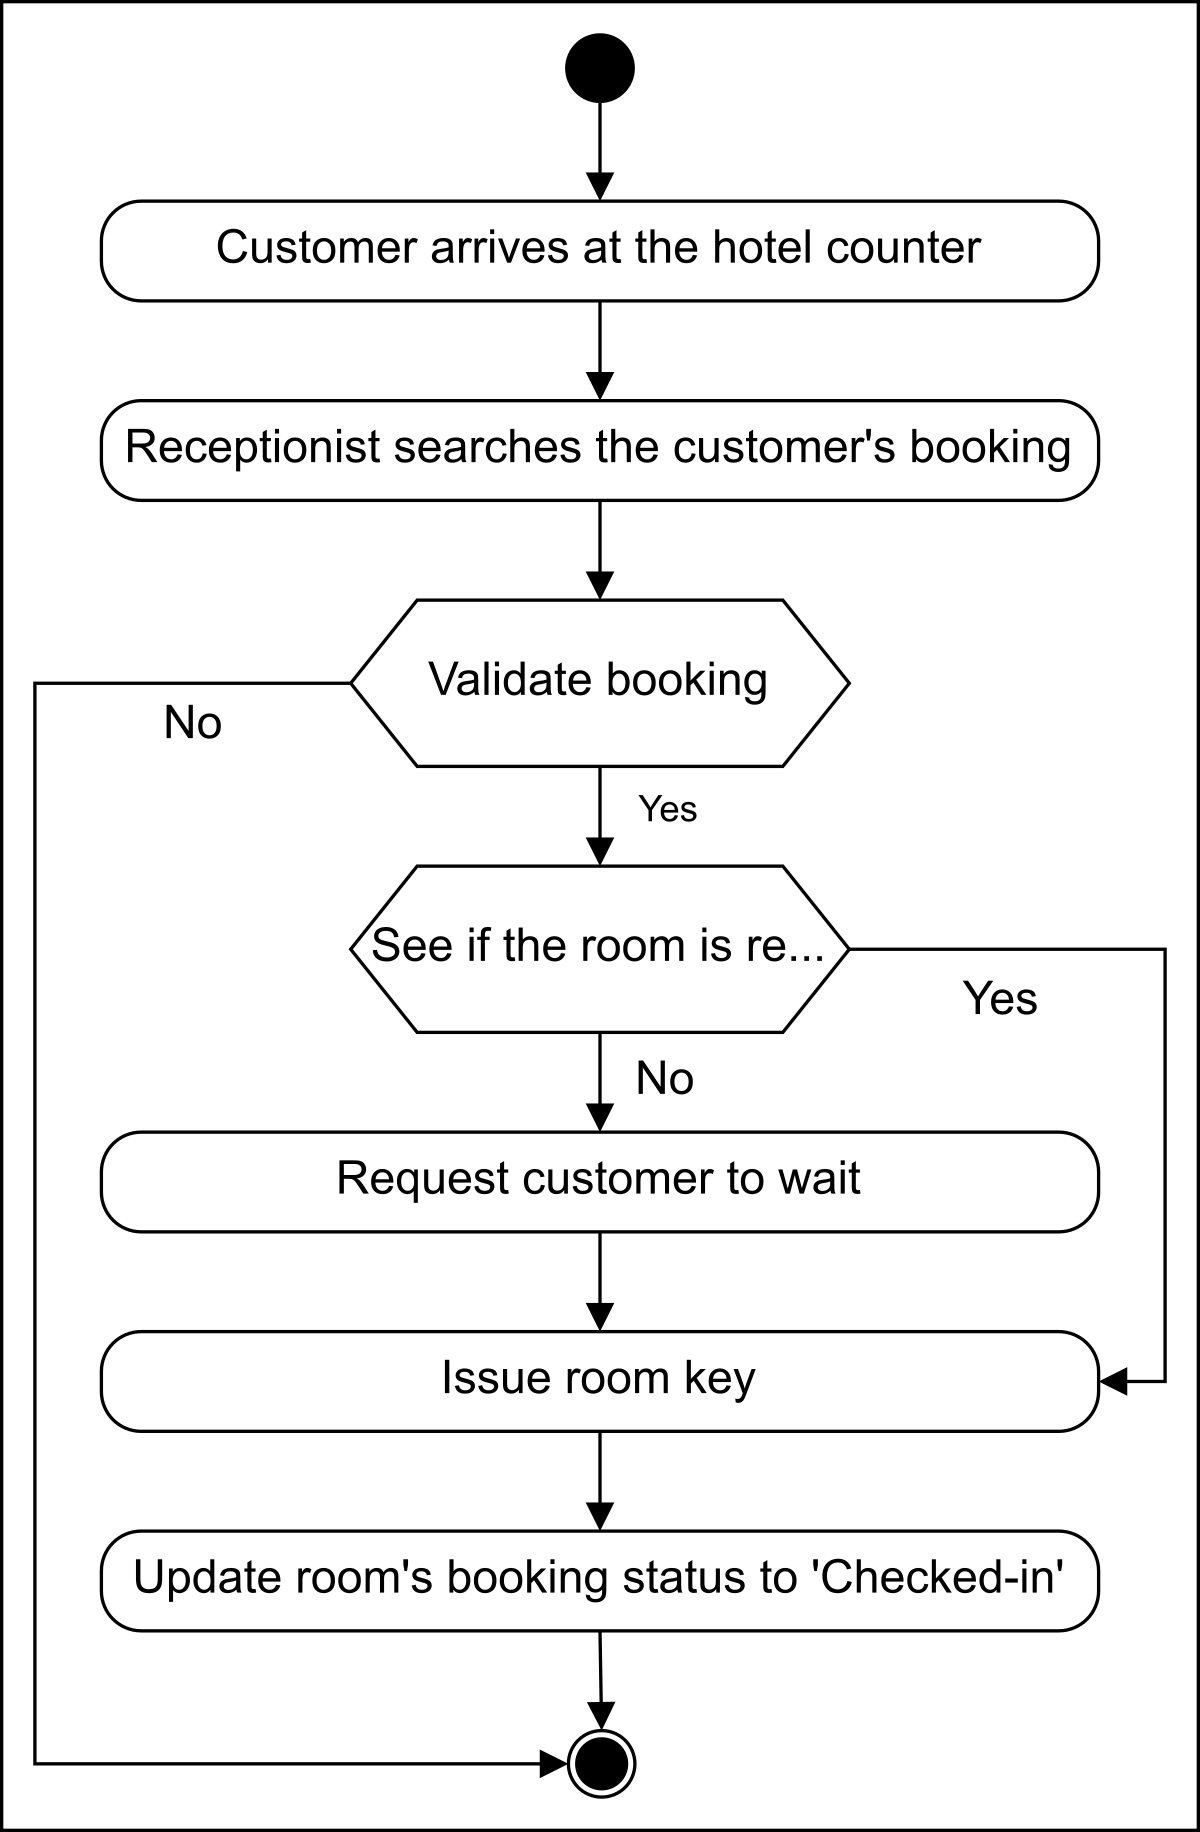
\includegraphics[width=0.5\textwidth]{Images/chapter_18/section_5412792868012032/5684483108110336.png}
 \caption{The activity diagram for the hotel check-in}
\end{figure}

\subsection{Activity challenge: Cancel a room booking}\label{qQ8UiLDWEEf6Cnibbq9TJ-2}
\\
You'll help us create an activity diagram of a customer who wants to cancel their room booking.
\\
A skeleton of the activity diagram is given below, provided that a guest will cancel the room booking from the hotel.

\begin{figure}[htbp]
 \centering
 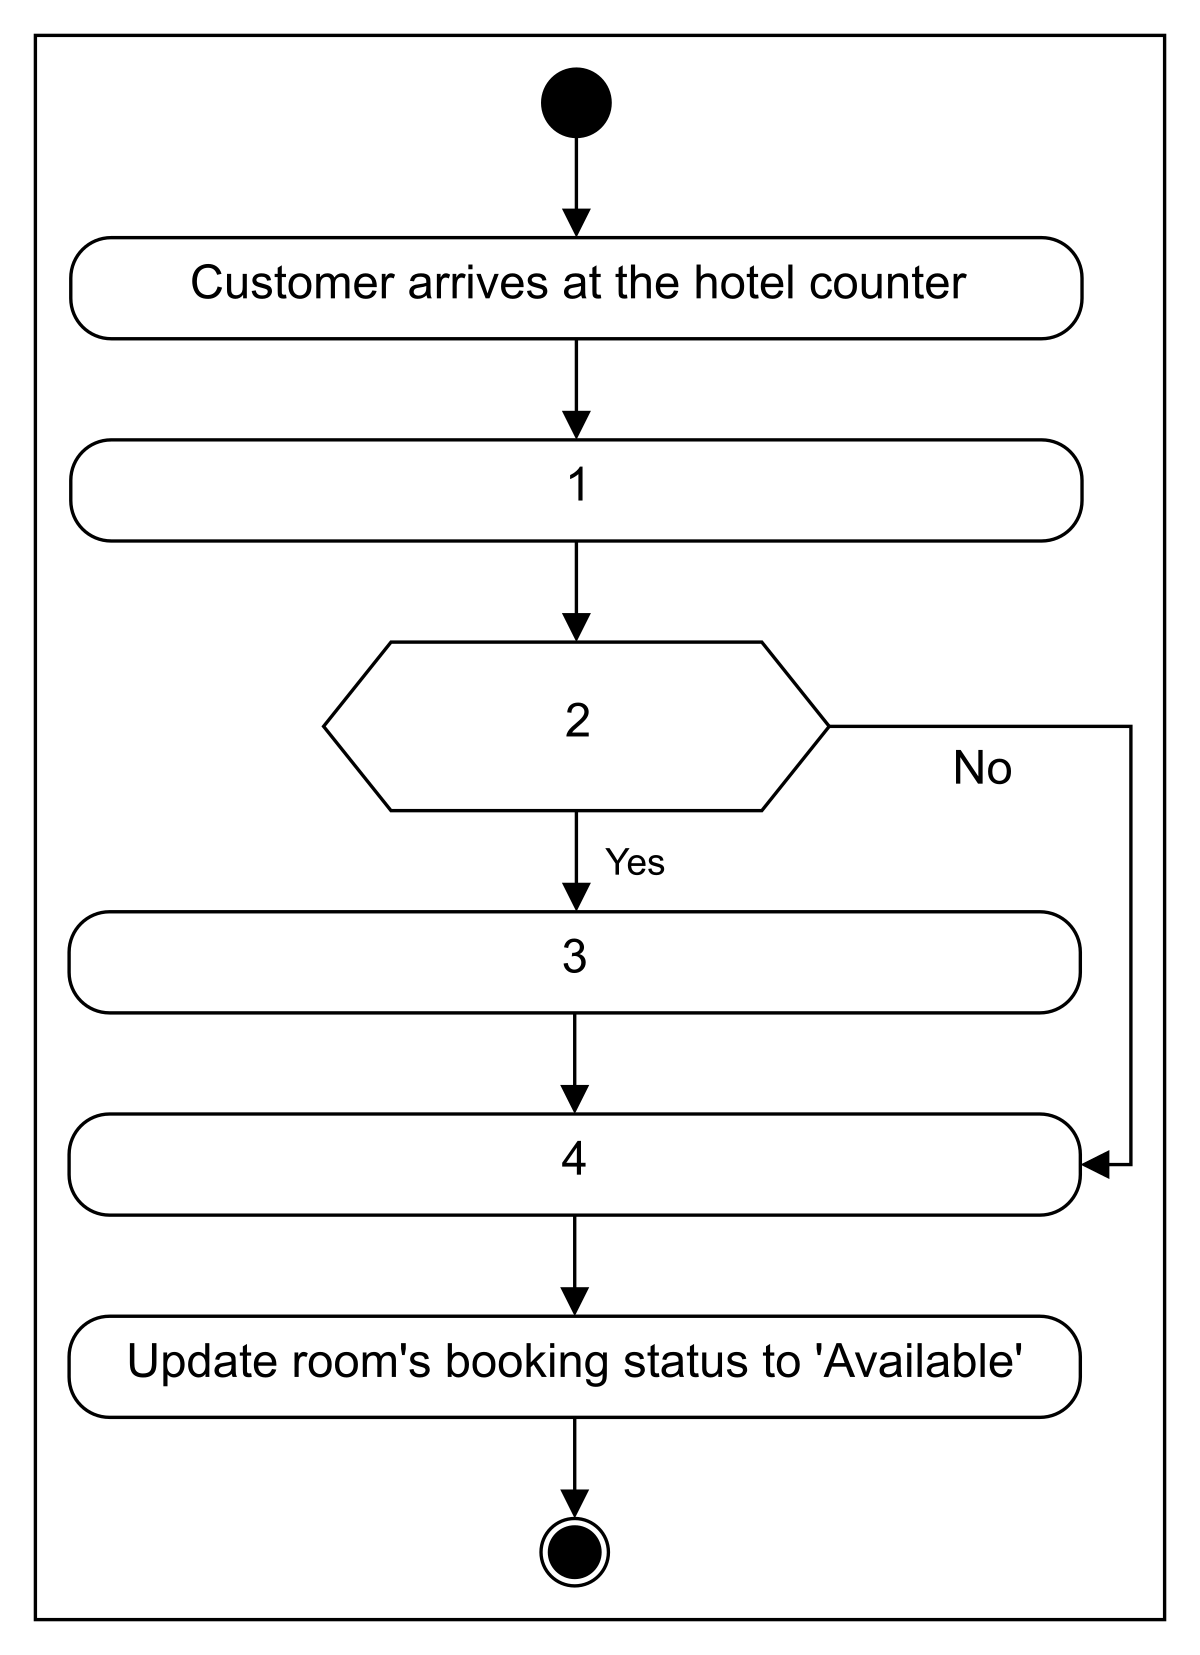
\includegraphics[width=0.5\textwidth]{Images/chapter_18/section_5412792868012032/4909796787355648.png}
 \caption{The activity diagram for booking cancellation}
\end{figure}

Notice that the actions in the diagram above are numbered from 1 to 4. The slots below represent the activities, and the arrows represent the flow from one activity to another. Can you rearrange the slots below in the correct order they should appear in the activity diagram above?
\begin{quote}
\textbf{Note:} If you're stuck, click the ``Show Solution'' button.
\end{quote}

Alternatively, you can click the ``Show complete diagram'' button below to see the complete activity diagram.

We've looked at some of the activity diagrams of our hotel management system. In the next lesson, we will present the code for our designed classes in some of the most popular languages.

% End of section content